\documentclass[tikz,border=10pt]{standalone}
\usepackage{tikz}
\usepackage{amsmath,amssymb}
\usetikzlibrary{positioning,fit,shapes.geometric,arrows.meta,calc,decorations.pathreplacing}

\begin{document}
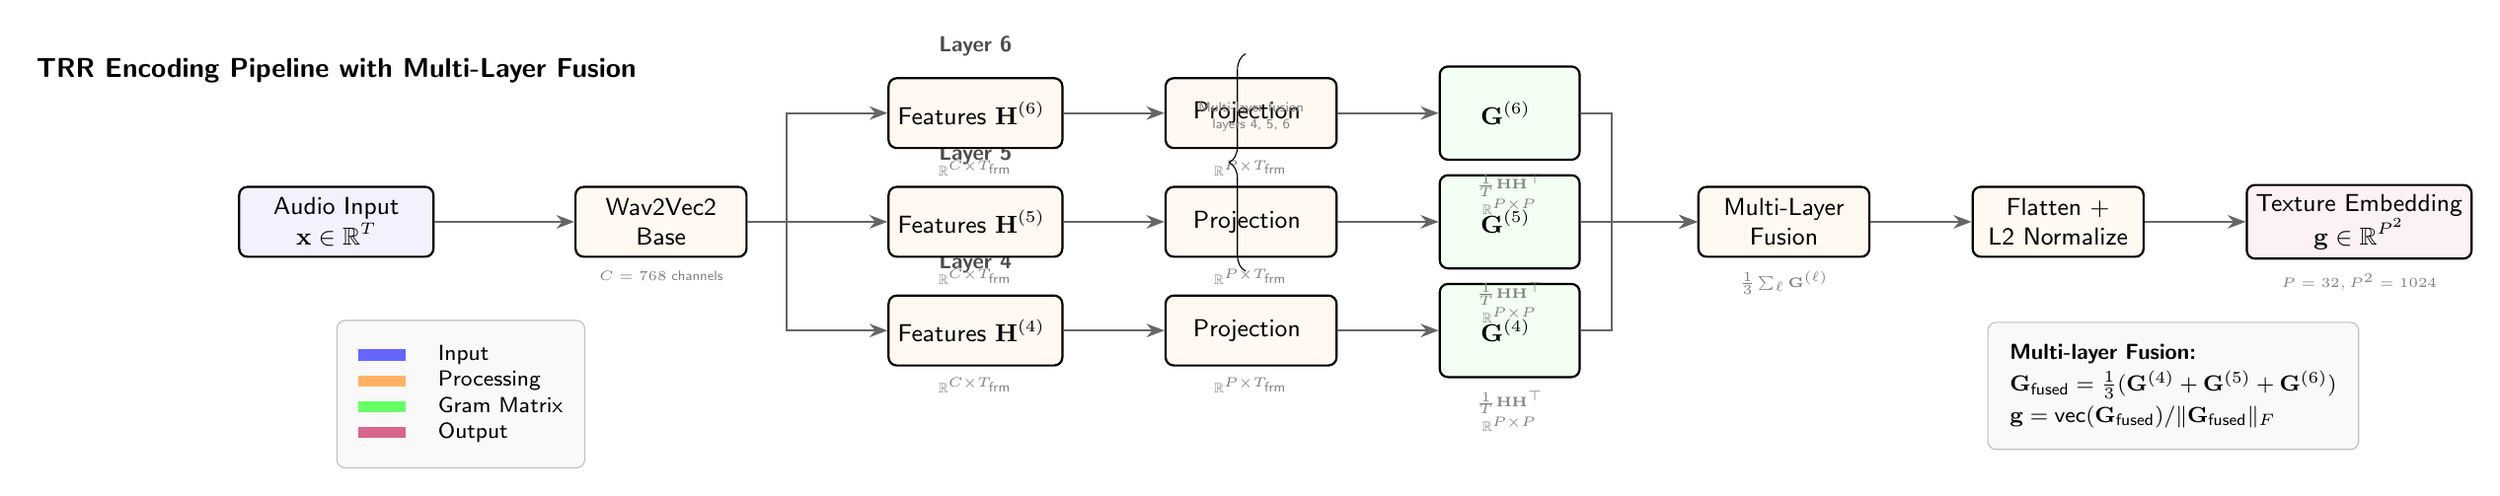
\begin{tikzpicture}[
    font=\sffamily\small,
    >=Stealth,
    box/.style={
        draw,
        rounded corners=3pt,
        minimum width=2.2cm,
        minimum height=0.9cm,
        align=center,
        fill=white,
        line width=0.8pt
    },
    inputbox/.style={
        box,
        fill=blue!5,
        minimum width=2.5cm
    },
    processbox/.style={
        box,
        fill=orange!5
    },
    matrixbox/.style={
        box,
        fill=green!5,
        minimum width=1.8cm,
        minimum height=1.2cm
    },
    outputbox/.style={
        box,
        fill=purple!5,
        minimum width=2.5cm
    },
    layerlabel/.style={
        font=\sffamily\footnotesize\bfseries,
        text=black!70
    },
    dimlabel/.style={
        font=\sffamily\tiny,
        text=black!50,
        align=center
    },
    arrow/.style={
        ->,
        line width=0.8pt,
        draw=black!60
    },
    brace/.style={
        decorate,
        decoration={brace,amplitude=6pt,raise=2pt}
    }
]

% Dimensions
\def\layersep{1.8cm}
\def\vsep{1.4cm}

% Input: Audio
\node[inputbox] (audio) {Audio Input\\$\mathbf{x} \in \mathbb{R}^{T}$};

% Wav2Vec2 Feature Extraction
\node[processbox, right=\layersep of audio] (wav2vec) {Wav2Vec2\\Base};
\node[dimlabel, below=0.05cm of wav2vec] {$C = 768$ channels};

% Three parallel layers
\foreach \i/\layer in {1/4, 2/5, 3/6} {
    % Feature map
    \node[processbox, right=\layersep of wav2vec, yshift={(\i-2)*\vsep}] (feat\i) {
        Features $\mathbf{H}^{(\layer)}$
    };
    \node[dimlabel, below=0.02cm of feat\i] {$\mathbb{R}^{C \times T_{\text{frm}}}$};

    % Projection
    \node[processbox, right=1.3cm of feat\i] (proj\i) {
        Projection
    };
    \node[dimlabel, below=0.02cm of proj\i] {$\mathbb{R}^{P \times T_{\text{frm}}}$};

    % Gram Matrix
    \node[matrixbox, right=1.3cm of proj\i] (gram\i) {
        $\mathbf{G}^{(\layer)}$
    };
    \node[dimlabel, below=0.05cm of gram\i] {$\frac{1}{T}\mathbf{H}\mathbf{H}^\top$\\$\mathbb{R}^{P \times P}$};

    % Layer label
    \node[layerlabel, above=0.15cm of feat\i] {Layer \layer};

    % Arrows
    \draw[arrow] (wav2vec.east) -- ++(0.5,0) |- (feat\i.west);
    \draw[arrow] (feat\i) -- (proj\i);
    \draw[arrow] (proj\i) -- (gram\i);
}

% Fusion
\node[processbox, right=1.5cm of gram2] (fusion) {Multi-Layer\\Fusion};
\node[dimlabel, below=0.05cm of fusion] {$\frac{1}{3}\sum_{\ell} \mathbf{G}^{(\ell)}$};

% Arrows from Gram matrices to Fusion
\draw[arrow] (gram1.east) -- ++(0.4,0) |- (fusion.west);
\draw[arrow] (gram2) -- (fusion);
\draw[arrow] (gram3.east) -- ++(0.4,0) |- (fusion.west);

% Flatten and Normalize
\node[processbox, right=1.3cm of fusion] (flatten) {Flatten +\\L2 Normalize};

% Output
\node[outputbox, right=1.3cm of flatten] (output) {Texture Embedding\\$\mathbf{g} \in \mathbb{R}^{P^2}$};
\node[dimlabel, below=0.05cm of output] {$P = 32, P^2 = 1024$};

% Arrows
\draw[arrow] (audio) -- (wav2vec);
\draw[arrow] (fusion) -- (flatten);
\draw[arrow] (flatten) -- (output);

% Braces for dimension reduction
\draw[brace] ([yshift=0.3cm]proj1.north) -- ([yshift=0.3cm]proj3.north)
    node[midway,above=8pt,dimlabel] {Multi-layer fusion\\layers 4, 5, 6};

% Title
\node[above=1.2cm of audio, font=\sffamily\bfseries\normalsize] (title) {
    TRR Encoding Pipeline with Multi-Layer Fusion
};

% Legend box
\node[below=0.8cm of audio, anchor=north west, font=\sffamily\footnotesize,
      draw=gray!50, rounded corners=3pt, inner sep=8pt, fill=gray!5] (legend) {
    \begin{tabular}{@{}ll@{}}
    \textcolor{blue!60}{\rule{0.6cm}{4pt}} & Input \\
    \textcolor{orange!60}{\rule{0.6cm}{4pt}} & Processing \\
    \textcolor{green!60}{\rule{0.6cm}{4pt}} & Gram Matrix \\
    \textcolor{purple!60}{\rule{0.6cm}{4pt}} & Output \\
    \end{tabular}
};

% Mathematical formulation box
\node[below=0.8cm of output, anchor=north east, font=\sffamily\footnotesize,
      draw=gray!50, rounded corners=3pt, inner sep=8pt, fill=gray!5, align=left] (formula) {
    \textbf{Multi-layer Fusion:}\\[2pt]
    $\mathbf{G}_{\text{fused}} = \frac{1}{3}(\mathbf{G}^{(4)} + \mathbf{G}^{(5)} + \mathbf{G}^{(6)})$\\[2pt]
    $\mathbf{g} = \text{vec}(\mathbf{G}_{\text{fused}}) / \|\mathbf{G}_{\text{fused}}\|_F$
};

\end{tikzpicture}
\end{document}
